% !TeX root = Features.tex
\documentclass[../Dissertation.tex]{subfiles}

\begin{document}

\section{Feature Overview}

\subsection{Parsing and syntax trees}
A C++17 library was created for parsing strings produced by the formal grammar on types (Figure \ref{fig:typegrammar}). This library also includes a parser for naturality types.

\subsection{Composition and unification}


\subsection{Petri net generation}
\subsection{Visualisation and the user interface}

\begin{figure}[H]
\begin{center}
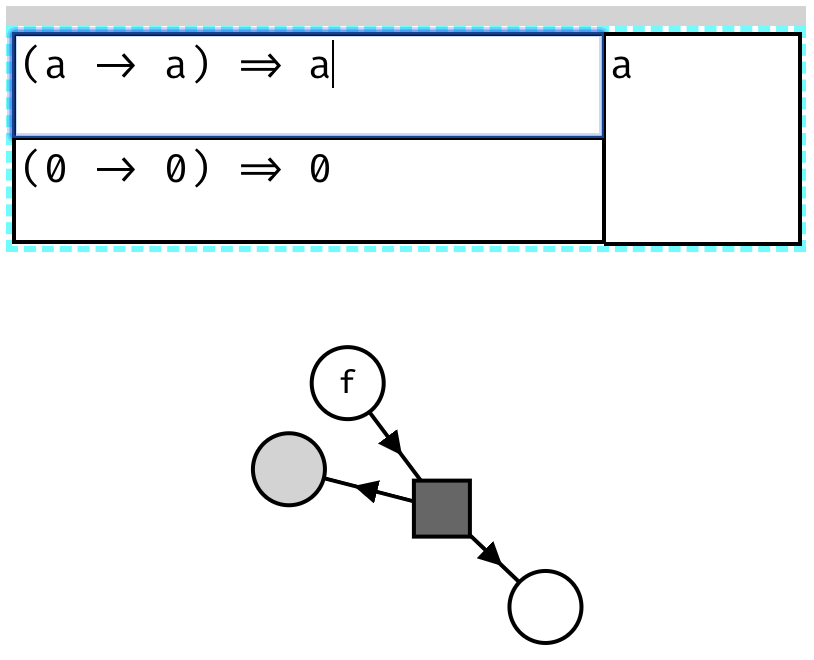
\includegraphics[scale=0.45]{component}
\end{center}
\caption{A single selected component.}
\label{fig:component}
\end{figure}

\begin{figure}[H]
\begin{center}
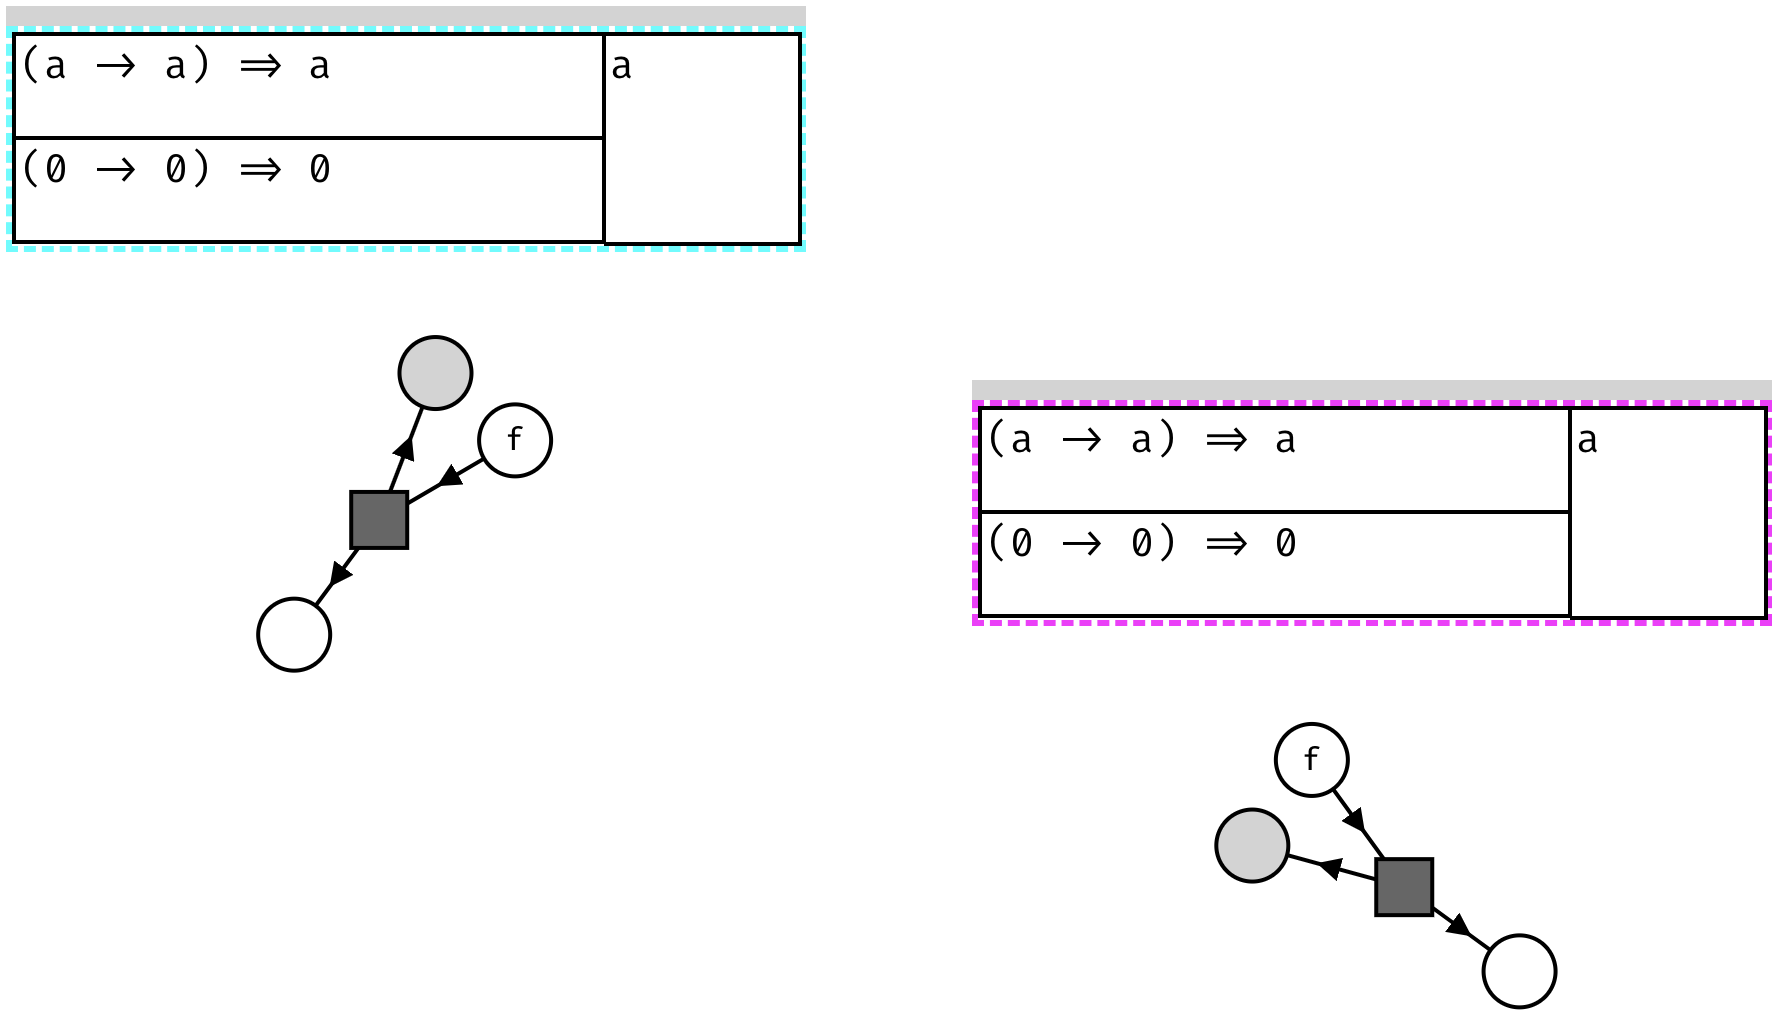
\includegraphics[scale=0.45]{selection}
\end{center}
\caption{Two selected components.}
\label{fig:selection}
\end{figure}

\begin{figure}[H]
\begin{center}
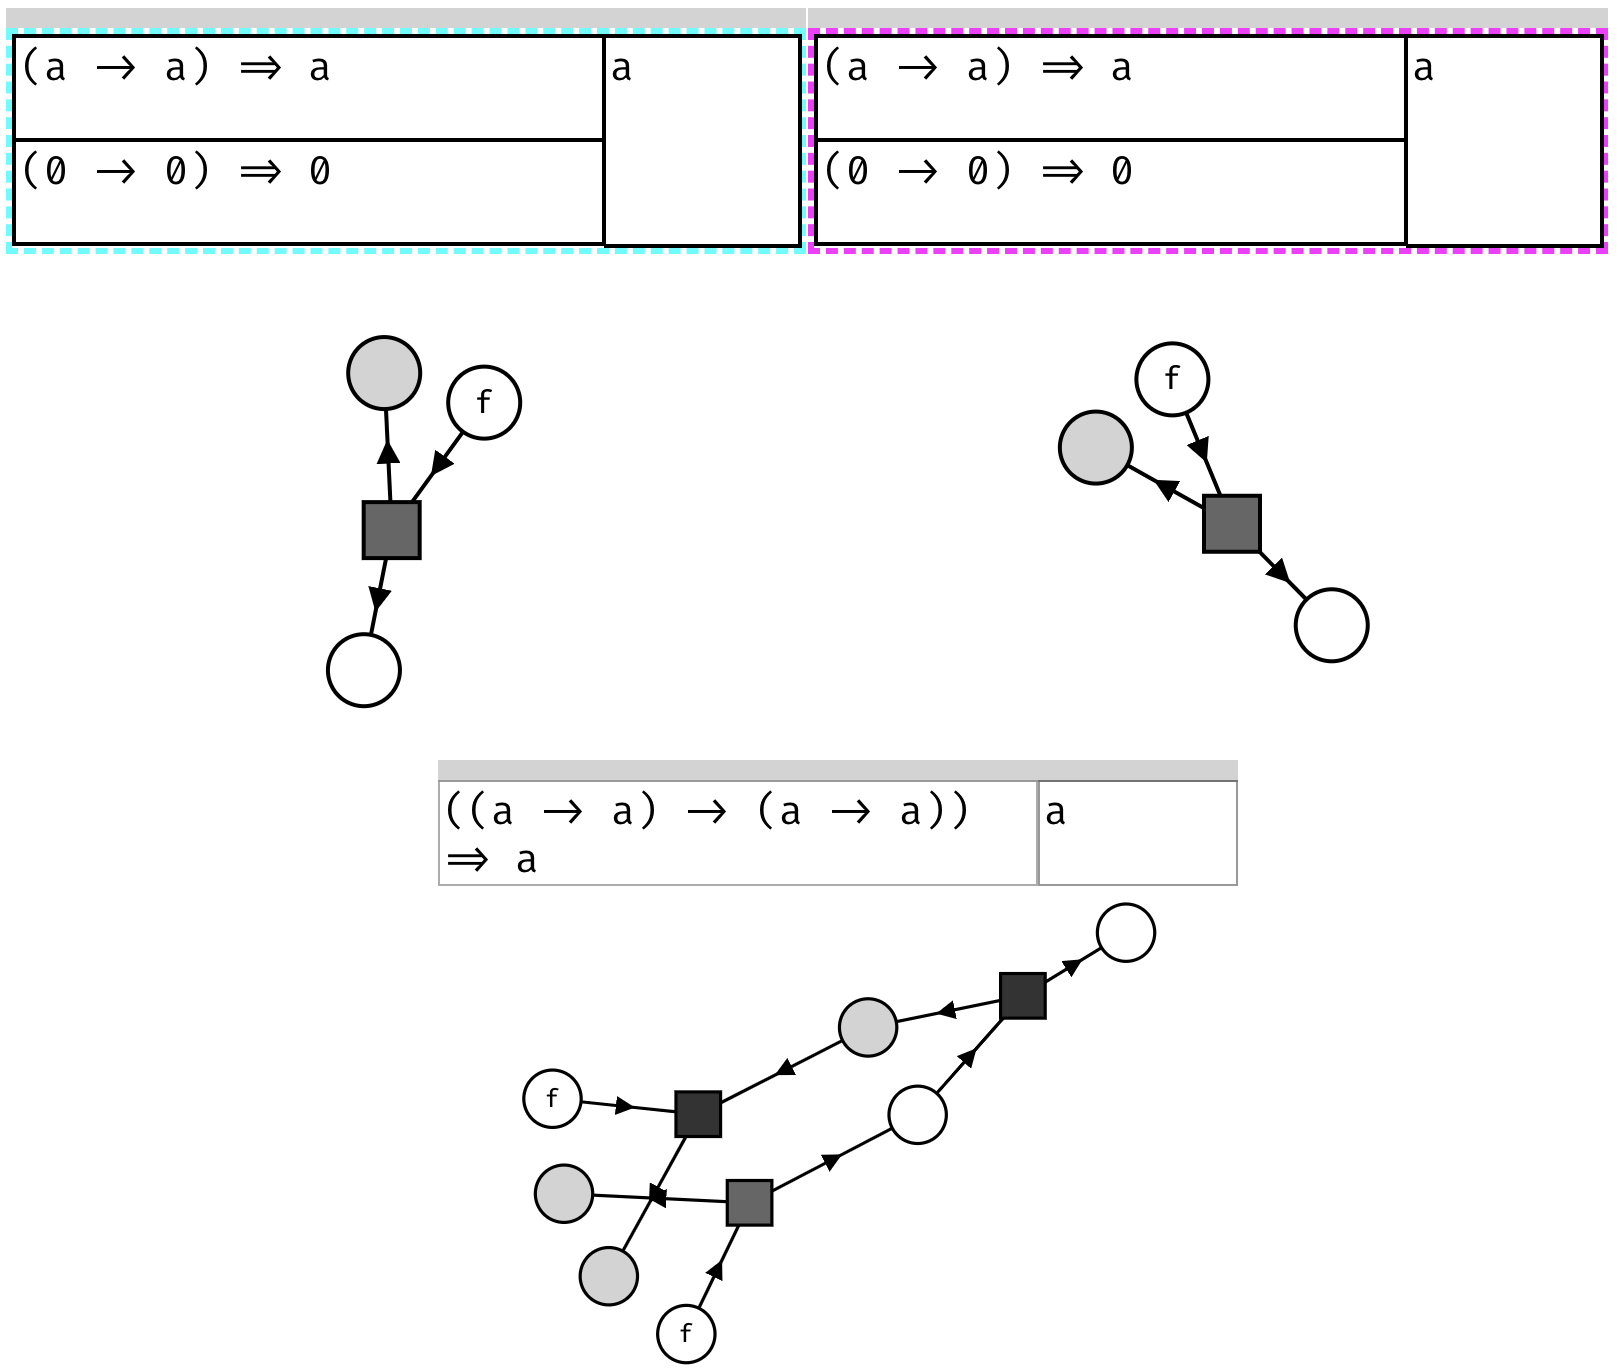
\includegraphics[scale=0.45]{compose1}
\end{center}
\caption{Two selected components and their composition.}
\label{fig:compose1}
\end{figure}

\begin{figure}[H]
\begin{center}
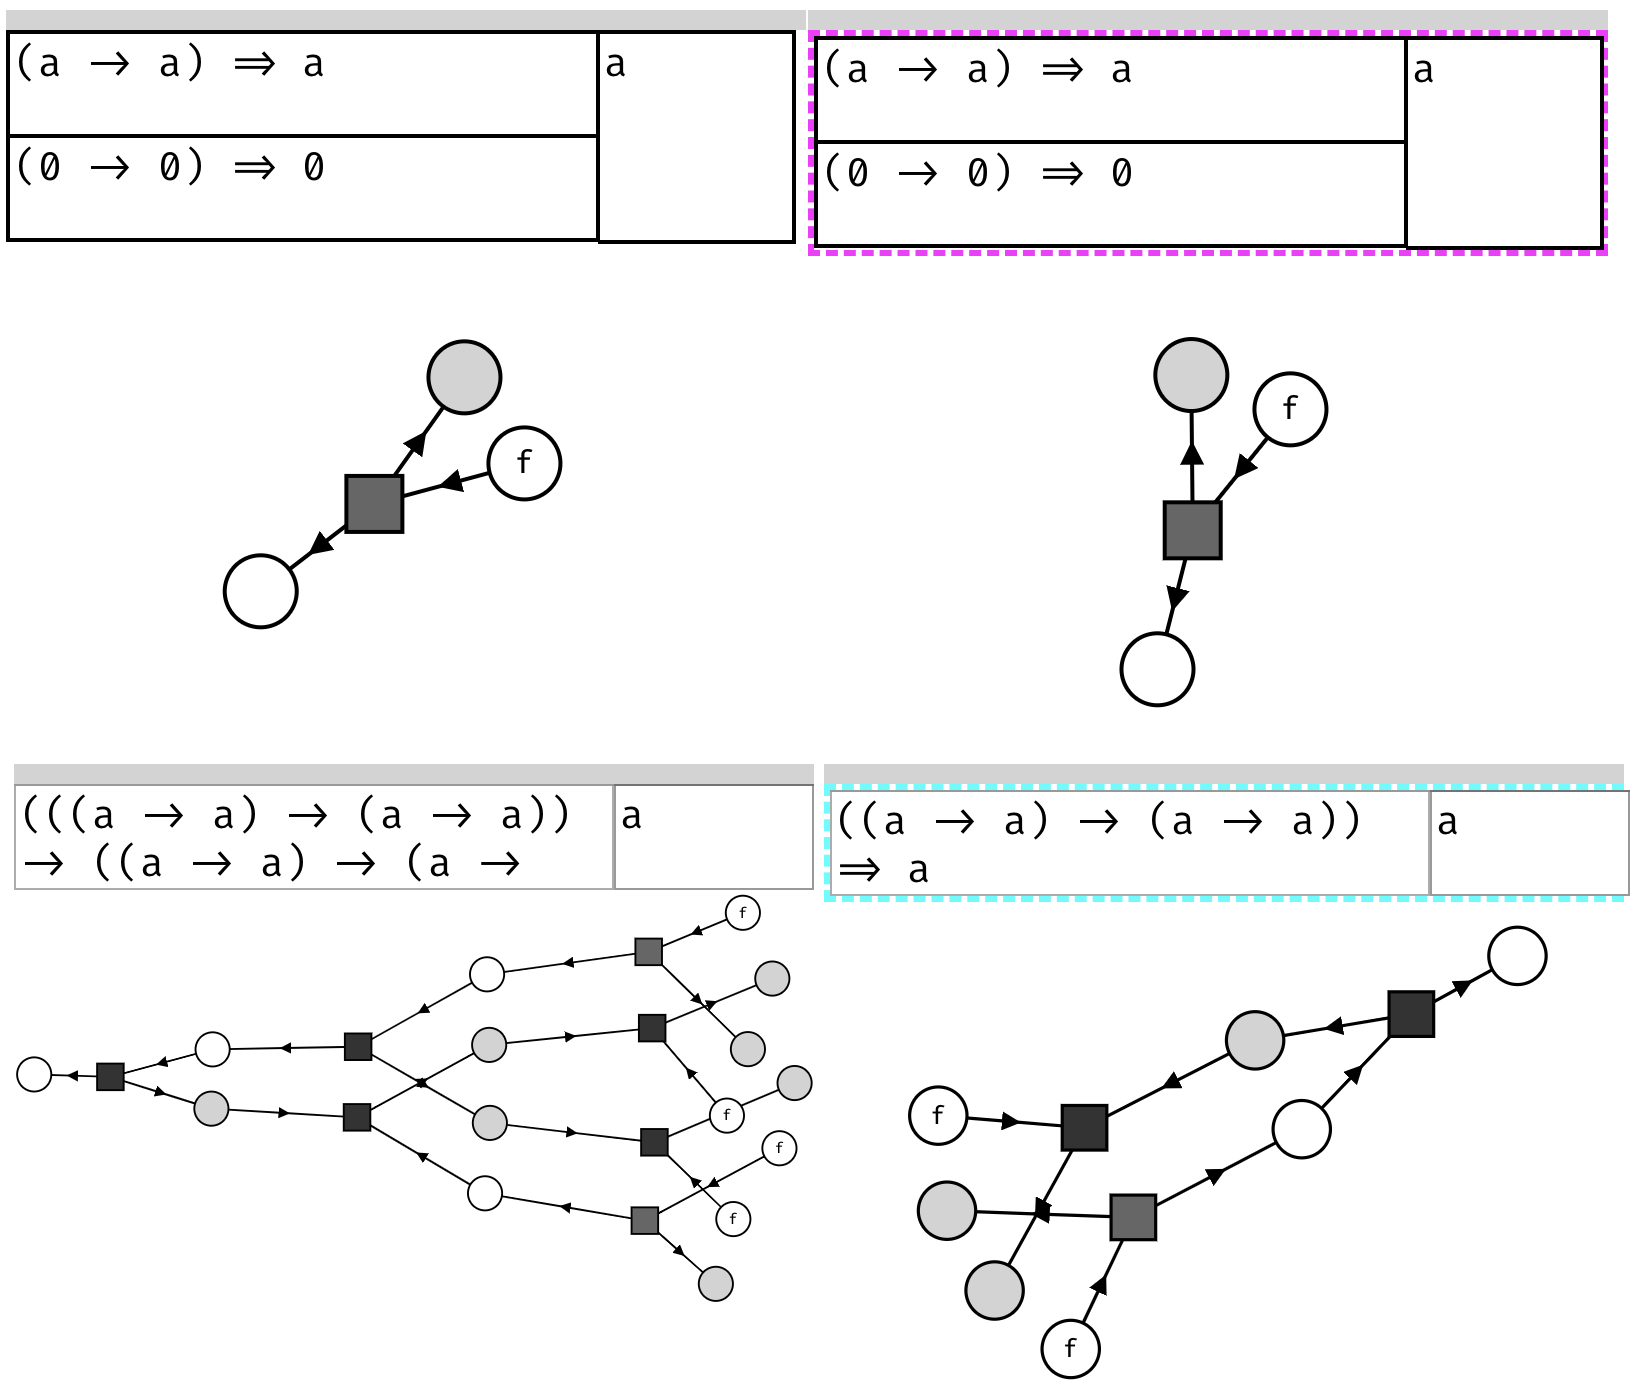
\includegraphics[scale=0.45]{compose2}
\end{center}
\caption{Generation of a Petri net by iterated composition.}
\label{fig:compose1}
\end{figure}

\subsection{Latex exporting}

\end{document}